\chapter{Chirality}
\label{ch:p2:chirality}

\readit{0}

\worktodo{
* Chirality
	* Chirality plot
	* Spectrum study plot
	* Coarse Dop condition plot -> done in numerics->cost
	* Eigen and Singular value decomps
	* G5 Hermiticity
	* Impl. chirality preservation -> done in lc->spin dof
	* Spectral study
	* All proofs I have so far
}


\worktodo{$[P,\chi^{5}]=0$, thus $P$ leaves the subspaces of fermion fields with definite chirality invariant.}

In this last chapter, we want to discuss the spin degrees of freedom that are carried over to the coarse grid.
There are many ways how this can be achieved.
We have already discussed some of them in \cref{sec:lc:spin}.
We want to formalize these findings more and come up with a necessary and sufficient condition for the coarse Dirac operator to have well-behaved spectrum.
To simplify things, we choose the Weyl basis for the $\gamma$-matrices because it makes chirality manifest,
\begin{align} \label{eq:gamma:weyl:basis}
\gamma_0 &=
\begin{pmatrix}
0 & 0 & 1 & 0 \\
0 & 0 & 0 & 1 \\
1 & 0 & 0 & 0 \\
0 & 1 & 0 & 0
\end{pmatrix} \;,
&
\gamma_1 &=
\begin{pmatrix}
0 & 0 & 0 & 1 \\
0 & 0 & 1 & 0 \\
0 & -1 & 0 & 0 \\
-1 & 0 & 0 & 0
\end{pmatrix} \\
\gamma_2 &=
\begin{pmatrix}
0 & 0 & 0 & -i \\
0 & 0 & i & 0 \\
0 & -i & 0 & 0 \\
i & 0 & 0 & 0
\end{pmatrix} \;,
&
\gamma_3 &=
\begin{pmatrix}
0 & 0 & 1 & 0 \\
0 & 0 & 0 & -1 \\
-1 & 0 & 0 & 0 \\
0 & 1 & 0 & 0
\end{pmatrix} \;.
\end{align}
This choice makes $\gamma^5$ diagonal as
\begin{equation}
\gamma^5 =
\gamma_0 \gamma_1 \gamma_2 \gamma_3 =
\begin{pmatrix}
1 & 0 & 0 & 0 \\
0 & 1 & 0 & 0 \\
0 & 0 & -1 & 0 \\
0 & 0 & 0 & -1
\end{pmatrix} \;.
\end{equation}
It acts on positive chirality as identity and on negative chirality as minus identity.
By this the \num{4} spin degrees of freedom of a Dirac spinor are divided into chiral and non-chiral ones.
This makes the chiral degree of freedom manifest in $\gamma^5$ and we can write it as tensor product
\begin{equation}
\gamma^5 = \chi^5 \otimes \id_S \;,
\qquad
\chi^5 = 
\sigma_3 = 
\begin{pmatrix}
1 & 0 \\
0 & -1
\end{pmatrix} \;,
\qquad
\id_S = 
\begin{pmatrix}
1 & 0 \\
0 & 1
\end{pmatrix} \;,
\end{equation}
where $\chi^5$ only acts on the chiral degrees of freedom and the identity $\id_S$ on the remaining spins.
Such a decomposition is also possible in the Dirac- or Majorana basis.
The chiral operator $\chi^5$ will then be a different Pauli matrix.

On the fine grid, the $\gamma^5$ operator only acts non-trivially on the spins.
We usually suppress the identities in the tensor product when acting in spinors and identify
\begin{equation}
\gamma^5 \equiv \id_{\idxspacetime} \otimes \gamma^5 \otimes \id_{\idxcolor} \;,
\end{equation}
where $\id_{\idxspacetime}$ and $\id_{\idxcolor}$ are identities acting on the spacetime and color degrees of freedom respectively.
In this chapter, we may leave the identities explicit for clarity and define the (separable) chiral operator acting on a spinor as
\begin{equation}
\Gamma^5 = \id_{\idxspacetime} \otimes \chi^5 \otimes \id_S \otimes \id_{\idxcolor} \;.
\end{equation}

\section{Coarse chirality}

Since $\Gamma^5$ is an operator acting on Dirac spinors
\begin{equation}
\Gamma^5 \colon \vslattice \longrightarrow \vslattice \;,
\end{equation}
we can coarsen it using the usual formula, \cref{eq:sd:coarse:op},
\begin{equation}
\coarse{\Gamma^5} = R \Gamma^5 T \colon \coarse{\vslattice} \longrightarrow \coarse{\vslattice} \;,
\end{equation}
where $R$ and $T$ are restrictor and prolongator defined in \cref{eq:R,eq:T}.
Similarly as with the fine operator, we can write the coarse operator as tensor product of identities with a (possibly) non-trivial chiral operator
\begin{equation}
\coarse{\Gamma^5} = \id_{\coarse{\idxspacetime}} \otimes \rho^5 \;,
\end{equation}
where $\id_{\coarse{\idxspacetime}}$ is the identity on the coarse spacetime and $\rho^{5}$ acts only on coarse spin and color indices.
%The identities themselves are not of interest, but the coarse chirality operator $\rho^5$ is.

As stated in \cref{sec:lc:spin} the spin degrees of freedom can be coarsened in many ways.
If we coarsen all of them, $N_s = 1$, then the two operators $\rho^{5}$ and $\id_{\coarse{S}}$ are both $1 \times 1$ matrices, i.e. numbers and the coarse $\coarse{\Gamma^5}$ is proportional to the identity.
If we coarsen none of them by leaving all \num{4} spins explicit on the coarse subspace $N_s = 4$, then both operators will be $2 \times 2$ matrices equal to their fine grid versions, $\rho^{5} = \chi^{5}$ and $\id_{\coarse{S}} = \id_S$.
Finally, if we coarsen using the chiral projectors \cref{eq:bootstrap:chiral} leaving the chiral indices explicit and coarsening the remaining spin indices $N_s=2$, we again find $\rho^{5} = \chi^{5}$ and $\id_{\coarse{S}} = 1$ as a number.
Alternatively we could coarsen the chiral indices and leave the non-chiral ones explicit.
This would analogously result in $\rho^{5} = 1$ and $\id_{\coarse{S}} = \id_S$.
\Cref{tab:spins} summarizes most of the sensible choices.
We see that some preserve the trace on the fine-grid $\tr(\Gamma^{5})=0$, some preserve chirality $[P, \Gamma^{5}] = 0$ and some preserve fine-grid low modes $P \evec_i = \evec_i$.

\begin{table}
\begin{tabular}{c|cccccc}
\toprule
i & $N_s$ & Spins & $\rho^{5}$ & $\tr(\rho^{5})$ & $[P, \Gamma^{5}]$ & $P\evec_i = \evec_i$ \\
\midrule
1 & 1 & - & Hermitian & $\in \mathbb{R}$ & $\neq 0$ & $\boxtimes$ \\
\midrule
2 & 2 & $P_{\pm} = \frac{1}{2} \left( \id \pm \gamma^{5} \right)$ & $\chi^{5} \otimes \id_{\coarse{\idxcolor}}$ & $0$ & $0$ & $\boxtimes$ \\
\midrule
3 & 2 & $P_i = \id, P_g = \gamma^{5}$ & $B \left(\chi^{5} \otimes \id_{\coarse{\idxcolor}} \right) B^{-1}$ & $0$  & $0$ & $\boxtimes$ \\
\midrule
4 & 2 &
%\(\displaystyle
\makecell{
	$P_{e} = P_0 + P_2$, \\
	$P_{o} = P_1 + P_3$
}
%(P_{1})_{[\alpha \beta]} = \delta_{\alpha \beta} \left( \delta_{\alpha 1} + \delta_{\alpha 3} \right)
%\)
& \worktodo{?} & \textcolor{red}{?} & \textcolor{red}{?} & $\boxtimes$ \\
\midrule
5 & 2 & $P_0, P_1$ & $+\id_{\coarse{S}} \otimes \id_{\coarse{\idxcolor}}$ & $+2 \Nc$ & $0$ & $\square$ \\
\midrule
6 & 2 & $P_2, P_3$ & $-\id_{\coarse{S}} \otimes \id_{\coarse{\idxcolor}}$ & $-2 \Nc$ & $0$ & $\square$ \\
\midrule
7 & 4 & $P_0, P_1, P_2, P_3$ & $\chi^{5} \otimes \id_{\coarse{S}} \otimes \id_{\coarse{\idxcolor}}$ & $0$ & $0$ & $\boxtimes$ \\
\bottomrule
\end{tabular}
\caption{\label{tab:spins}
Projectors together with their number of coarse spin degrees of freedom $N_s$ and the form of coarse chiral and non-chiral operators. The table uses the definition of the spin projectors $(P_{\sigma})_{[\alpha \beta]} = \delta_{\alpha \beta} \delta_{\alpha \sigma}$ for $\sigma=0,1,2,3$. The matrix $B$ is some irrelevant change-of-basis matrix.
}
\end{table}

We want to further investigate the properties of the coarse chirality operator $\coarse{\Gamma^{5}}$.
For this we look at its eigenvalues and eigenvectors,
\begin{equation}
\coarse{\Gamma^{5}} \coarse{\psi} = \lambda \coarse{\psi} \;.
\end{equation}
Plugging in the definitions of the coarse objects, we obtain
\begin{equation}
R \Gamma^{5} \psi = \lambda R \psi \;,
\end{equation}
where we used $P = TR$ and the fact that for every coarse spinor $\coarse{\psi}$ we have $P \psi = \psi$ for its prolonged spinor $\psi = T \coarse{\psi}$.
This is just an equation restricted to the subspace and we can prolong it to the fine grid by applying $T$ to both sides,
\begin{equation}
P \Gamma^{5} \psi = \lambda \psi \;.
\end{equation}
We will now use a property which will be discussed later, $[P, \Gamma^{5}] = 0$, and find the eigenvalue equation for the fine-grid chirality operator $\Gamma^{5} \psi = \lambda \psi$.
Therefore, if $[P, \Gamma^{5}] = 0$ the spectrum of the coarse chirality operator is a subset of the fine one; either
\begin{equation} \label{eq:sigma}
\sigma(\coarse{\Gamma^{5}}) = \{+1\} \;,
\qquad
\sigma(\coarse{\Gamma^{5}}) = \{-1\} \;,
\qquad
\text{or}
\qquad
\sigma(\coarse{\Gamma^{5}}) = \{+1, -1\} \;.
\end{equation}
Clearly for the first two spectra the coarse chirality operator will be proportional to the identity and will not be traceless corresponding to cases $i=5,6$ in \cref{tab:spins}.
A trace-preserving operator appears if both eigenspaces of the fine chirality operator are used symmetrically when coarsening.

% We will continue with defining the \df{net-chirality} of a field by the number
% \begin{equation}
% \chi(\psi) = \frac{\psi^{\dagger} \Gamma^{5} \psi}{\psi^{\dagger} \psi} \in [-1, 1] \;.
% \end{equation}
% The set of values for all possible $\psi \in \vslattice$ is the \df{numerical range},
% \begin{equation}
% W(\Gamma^{5}) = \left\{ \frac{\psi^\dagger \Gamma^{5} \psi}{\psi^{^\dagger} \psi} \; \middle| \; \psi \in \vslattice \right\} = [-1, 1] \;.
% \end{equation}
% This implies that if $\chi(\psi) > 0$ the field is biased toward right-handed and if $<0$ towards left-handed chirality.

\begin{lemma} \label{lemma:chirality:preservation:equiv}
Assuming that $P$ and $\Gamma^{5}$ are Hermitian, the following statements are all equivalent:
\begin{align}
[P, \Gamma^{5}] &= 0 \;, \label{eq:lemma:chirality:preservation:equiv} \\
\sigma(\coarse{\Gamma^{5}}) &\subseteq \sigma(\Gamma^{5}) \;, \label{eq:lemma:sigma} \\
(\coarse{\Gamma^{5}})^{2} &= \id \;, \label{eq:lemma:involution} \\
\tr([P, \Gamma^{5}]^{2}) &= 0 \label{eq:lemma:trsq0} \;.
\end{align}
\end{lemma}
\begin{proof}
Assuming the first equality to be true, we have already shown that the spectrum has to be one of \cref{eq:sigma}.
Thus \cref{eq:lemma:chirality:preservation:equiv} implies \cref{eq:lemma:sigma}.

Looking at an operator with one of the three possible spectra, all of them square to an operator with spectrum $\{1\}$, which is the identity operator.
Thus \cref{eq:lemma:sigma} implies \cref{eq:lemma:involution}.

Assuming we have an involution, we calculate straight,
\begin{align}
\tr([P, \Gamma^{5}]^{2})
&= 2 \left[ \tr(P \Gamma^{5} P \Gamma^{5})  - \tr(P) \right] \\
&= 2 \left[ \tr(R \Gamma^{5} T R \Gamma^{5} T)  - \rank(P) \right] \\
&= 2 \left[ \tr( \coarse{\Gamma^{5}} \coarse{\Gamma^{5}} )  - \dim(\coarse{\vslattice}) \right] \\
&= 2 \left[ \tr( \id )  - \dim(\coarse{\vslattice}) \right] \\
&= 0 \;,
\end{align}
where in the last step we used the involution property of $\coarse{\Gamma^{5}}$.
Thus \cref{eq:lemma:involution} implies \cref{eq:lemma:trsq0}.

Finally, assuming \cref{eq:lemma:trsq0} and Hermiticity of $P$ and $\Gamma^{5}$, we find that
\begin{equation}
[P, \Gamma^{5}]^{\dagger} = - [P, \Gamma^{5}] \;,
\end{equation}
is skew-Hermitian.
Its eigenvalues are pure imaginary, $\sigma([P, \Gamma^{5}]) = \{ i \lambda_j\}_j$ for $\lambda_j \in \mathbb{R}$.
The trace over the operator squared is zero by assumption, thus
\begin{equation}
0 = \sum_{j} (i \lambda_j)^2 = - \sum_{j} \lambda_j^2 \;.
\end{equation}
This is only possible if $\lambda_j=0$ for all $j$.
Thus \cref{eq:lemma:trsq0} implies \cref{eq:lemma:chirality:preservation:equiv} concluding the proof.
\end{proof}

\section{Numerical range}

Before we analyze coarsenings and operators, we need the definition of numerical range.
The \df{numerical range} of an operator $A \colon \vslattice \rightarrow \vslattice$ is defined as
\begin{align} \label{eq:def:numerical:range}
W(A) \coloneqq \left\{ \psi^\dagger A \psi \; \middle| \; \psi \in \vslattice \; \text{and} \; \norm{\psi} = 1 \right\}.
\end{align}

The numerical range of an operator on the fine grid is related to the numerical range of the coarse operator.

\begin{theorem}[Numerical range of coarse operators] \label{thm:numerical:range}
Assume $K$ to be an operator acting on the fine-grid lattice, $K \colon \vslattice \rightarrow \vslattice$ and $\coarse{K}$ a coarsening of $K$ acting on the coarse grid, $\coarse{K} \colon \coarse{\vslattice} \rightarrow \coarse{\vslattice}$.
Then
\begin{equation}
W(\coarse{K}) \subseteq W(K) \;.
\end{equation}
\end{theorem}

\begin{proof}
We look at the numerical range of the coarse operator
\begin{align*}
W({\coarse{K}})
&= \left\{ \coarse{\psi}^\dagger \coarse{K} \coarse{\psi} \; \middle| \; \coarse{\psi} \in \coarse{\vslattice} \; \text{and} \; \norm{\coarse{\psi}} = 1 \right\} \\
&= \left\{ (\restrictor \psi)^\dagger \coarse{K} (\restrictor \psi) \; \middle| \; \psi \in \vslattice \; \text{and} \; \norm{\restrictor \psi} = 1 \; \text{and} \; P \psi = \psi \right\} \\
&= \left\{ \psi^\dagger \prolongator \restrictor K \prolongator \restrictor \psi \; \middle| \; \psi \in \vslattice \; \text{and} \; \norm{\restrictor \psi} = 1 \; \text{and} \; P \psi = \psi \right\}
\end{align*}
where we've used that $\restrictor^\dagger = \prolongator$. We use that $P = P^\dagger = \prolongator \restrictor$ and $\norm{\restrictor \psi} = (\restrictor \psi)^\dagger \restrictor \psi = \psi^\dagger P \psi = \norm{\psi}$ if $P \psi = \psi$ and find
\begin{align*}
W({\coarse{K}})
&= \left\{ \psi^\dagger K \psi \; \middle| \; \psi \in \vslattice \; \text{and} \; \norm{\psi} = 1 \; \text{and} \; P \psi = \psi \right\} \\
&\subseteq \left\{ \psi^\dagger K \psi \; \middle| \; \psi \in \vslattice \; \text{and} \; \norm{\psi} = 1 \right\} \\
&= W({K}).
\end{align*}
\end{proof}

Importantly, this result holds for every imaginable coarsening of $K$.
We continue with some properties about numerical ranges of operators.

\begin{lemma}[] \label{lemma:symmetric:numerical:range}
Assume $K$ be an operator acting on the fine-grid lattice and to be $\Gamma^{5}$-Hermitian, i.e. $K^{\dagger} = \Gamma^{5} K \Gamma^{5}$.
Then the numerical range of $K$ is symmetric about the real axis,
\begin{equation}
W(K) = W(K)^{\star} \iff \forall z \in W(K) \colon \bar{z} \in W(K) \;.
\end{equation}
\end{lemma}

\begin{proof}
Clearly we have $W(K^{\dagger}) = W(K)^{\star}$ and $W(K^{\dagger}) = W(\Gamma^{5} K (\Gamma^{5})^{\dagger}) = W(K)$, since $\Gamma^{5}$ is unitary.
\end{proof}

By substituting $K=D$, \cref{lemma:symmetric:numerical:range} implies that the numerical range of the Wilson-Clover Dirac operator $D$ is symmetric about the real axis, just as its eigenvalues are.

\section{Simple operators}

First, we will look at coarsenings of Hermitian positive definite (HPD) systems.
They form the easiest class of operators and we will analytically proof that for such an operator $\kappa(\coarse{K}) \leq \kappa(K)$, irrespective of how it is coarsened.

\begin{theorem}[Condition of coarse HPD operators] \label{thm:cond:hpd}
Assume $K$ to be a Hermitian positive definite operator acting on the fine-grid lattice, $K \colon \vslattice \rightarrow \vslattice$. Then the condition number of the coarse-grid operator $\coarse{K}$ is bound from above by the condition number of the fine-grid operator,
\begin{equation}
\kappa(\coarse{K}) \leq \kappa(K) \;.
\end{equation}
\end{theorem}

\begin{proof}
$K$ is Hermitian and positive definite, thus invertible: $\forall \lambda \in \sigma(K)$ we have $\lambda > 0$.
% We define the \df{numerical range} of an operator $A \colon \vslattice \rightarrow \vslattice$ as
% \begin{align} \label{eq:def:numerical:range}
% W(A) \coloneqq \left\{ \psi^\dagger A \psi \; \middle| \; \psi \in \vslattice \; \text{and} \; \norm{\psi} = 1 \right\}.
% \end{align}
The numerical range of $K$ is the interval in $\mathbb{R}_+$ delimited by the smallest and largest eigenvalue of $K$~\cite{gustafson1997numerical}, i.e. $W(K) = [ \lambda_{min}, \lambda_{max} ] \subset \mathbb{R}_+$.
% Then
% \begin{align*}
% W({\coarse{K}})
% &= \left\{ \coarse{\psi}^\dagger \coarse{K} \coarse{\psi} \; \middle| \; \coarse{\psi} \in \coarse{\vslattice} \; \text{and} \; \norm{\coarse{\psi}} = 1 \right\} \\
% &= \left\{ (\restrictor \psi)^\dagger \coarse{K} (\restrictor \psi) \; \middle| \; \psi \in \vslattice \; \text{and} \; \norm{\restrictor \psi} = 1 \; \text{and} \; P \psi = \psi \right\} \\
% &= \left\{ \psi^\dagger \prolongator \restrictor K \prolongator \restrictor \psi \; \middle| \; \psi \in \vslattice \; \text{and} \; \norm{\restrictor \psi} = 1 \; \text{and} \; P \psi = \psi \right\}
% \end{align*}
% where we've used that $\restrictor^\dagger = \prolongator$. We use that $P = P^\dagger = \prolongator \restrictor$ and $\norm{\restrictor \psi} = (\restrictor \psi)^\dagger \restrictor \psi = \psi^\dagger P \psi = \norm{\psi}$ if $P \psi = \psi$ and find
% \begin{align*}
% W({\coarse{K}})
% &= \left\{ \psi^\dagger K \psi \; \middle| \; \psi \in \vslattice \; \text{and} \; \norm{\psi} = 1 \; \text{and} \; P \psi = \psi \right\} \\
% &\subseteq \left\{ \psi^\dagger K \psi \; \middle| \; \psi \in \vslattice \; \text{and} \; \norm{\psi} = 1 \right\} \\
% &= W({K}).
% \end{align*}
Defining the smallest and largest eigenvalue of $\coarse{K}$ as $\mu_{min}$ and $\mu_{max}$ respectively, we use \cref{thm:numerical:range} and find $[ \mu_{min}, \mu_{max}] \subseteq [ \lambda_{min}, \lambda_{max} ]$, thus $\mu_{min} \geq \lambda_{min} > 0$ and $0 < \mu_{max} \leq \lambda_{max}$, which directly implies $\kappa(\coarse{K}) \leq \kappa(K)$, since all eigenvalues are positive. As a consequence, $\coarse{K}$ is HPD as well.
\end{proof}

\Cref{thm:cond:hpd} shows that with a HPD operator we do not need to care about how to coarsen.
Coarse operators are better conditioned in \emph{every} case.
Meaning that one can always coarsen $D^{\dagger} D$ instead of $D$ safely.
However, this operator is now next-to-nearest neighbor and its coarse variant $\coarse{D^{\dagger} D}$ is significantly less sparse and harder to implement efficiently.
Nevertheless this has been done in the field~\cite{Cohen:2011ivh,Boyle:2014rwa}.
We continue with slightly more general operators.

\begin{theorem}[Condition of coarse normal, positively stable operators] \label{thm:cond:normal:pos:stable}
Assume $K$ to be a normal, $\Gamma^{5}$-Hermitian, positively stable ($\forall \lambda \in \sigma(B) \; : \; \Re{\lambda} > 0$) operator acting on the fine-grid lattice, $K \colon \vslattice \rightarrow \vslattice$, whose eigenvalue with smallest magnitude is real.
Then the condition number of the coarse-grid operator $\coarse{K}$ is bound from above by the condition number of the fine-grid operator,
\begin{equation}
\kappa(\coarse{K}) \leq \kappa(K) \;.
\end{equation}
\end{theorem}

\begin{proof}
If $K$ is normal, its numerical range equals to the convex hull of its spectrum, $W(K) = \text{conv}\{\sigma(K)\}$, which in turn is symmetric about the real axis using \cref{lemma:symmetric:numerical:range}.
Thus $\sigma(\coarse{K}) \subseteq \text{conv}\{\sigma(K)\}$ and the element of smallest magnitude of $\text{conv}\{\sigma(K)\}$ is the real part of the eigenvalue of $K$ with smallest magnitude.
By assumption this eigenvalue is real.
Its largest element in magnitude is always smaller or equal to the eigenvalue of $K$ with largest magnitude.
Therefore $\kappa(\coarse{K}) \leq \kappa(K)$.
\end{proof}

If the smallest magnitude eigenvalue of $K$ is not real, but complex in general, then the smallest magnitude element of $\text{conv}\{\sigma(K)\}$ is given by the real part of the smallest magnitude eigenvalue instead.
We then cannot guarantee anymore that the smallest magnitude eigenvalue of $\coarse{K}$ is not smaller than the one of $K$.
At least, we have the guarantee that $\coarse{K}$ is invertible, because $0 \not\in \text{conv}\{\sigma(K)\}$, a consequence of $K$ being positively stable.

\section{Chirality preservation}

Even though we know that the property of chirality preservation $[P, \Gamma^{5}]=0$ is not sufficient for the coarse operator to be well-conditioned, it is worth inspecting it further.

\begin{lemma}[Implications of chirality preservation] \label{lemma:chirality:preservation:implications}
Assuming chirality preservation $[P, \Gamma^{5}]=0$ and $K$ is a $\Gamma^{5}$-Hermitian operator on the fine-grid lattice, then it holds
\begin{align}
\coarse{\Gamma^{5}} \coarse{K} &= \coarse{\Gamma^{5} K} \;, \\
\coarse{K} \coarse{\Gamma^{5}} &= \coarse{K \Gamma^{5}} \;, \\
\coarse{K} \; \text{is} \; &\coarse{\Gamma^{5}} \text{-Hermitian.}
\end{align}
\end{lemma}

\begin{proof}
The first equation is readily shown as
\begin{align}
\coarse{\Gamma^{5}} \coarse{K} = R \Gamma^{5} T R K T = R \Gamma^{5} P K T = R P \Gamma^{5} K T = R \Gamma^{5} K T = \coarse{\Gamma^{5} K} \;.
\end{align}
The second equation is just the same again, and for the third equation we note that Hermiticity is preserved when coarsening and since $\Gamma^{5} K$ is Hermitian by assumption, so is $\coarse{\Gamma^{5} K}$ and $\coarse{\Gamma^{5}} \coarse{K}$, thus $\coarse{K}^{\dagger} = \Gamma^{5} \coarse{K} \Gamma^{5}$.
\end{proof}

These are properties we may wish to have on the coarse grid, but we note that for cases $i=5,6$ in \cref{tab:spins} this is satisfied  although not working as expected.

\subsection{Singular value decomposition}

On the fine-grid, the singular value decomposition of a $\Gamma^{5}$-Hermitian operator $K$ is
\begin{equation} \label{eq:svd}
K = \sum_{i} \lvert \lambda_i \rvert (\Gamma^{5} \psi_i) \tilde{\psi}_i^{\dagger} \;,
\end{equation}
where the $\psi_i$ and $\lambda_i$ are eigenmodes and eigenvalues of the Hermitian operator $\Gamma^{5} K$ and $\tilde{\psi}_i = \text{sign}(\lambda_i) \psi_i$.
%The magnitudes of the eigenvalues $\lvert \lambda_i \rvert$ are the singular values of $K$.
The singular values $\sigma_i = \lvert \lambda_i \rvert$ are the magnitudes of eigenvalues $\lambda_i$ of $\Gamma^{5} K$.

\begin{lemma}[Coarse singular value decomposition] \label{lemma:svd:coarse}
If chirality is preserved, $[P, \Gamma^5]=0$, the singular value decomposition of $\coarse{K}$ is equivalent to \cref{eq:svd}, but every operator and vector hatted.
\end{lemma}

\begin{proof}
Chirality preservation implies $\coarse{\Gamma^{5}}$-Hermiticity of $\coarse{K}$ and $\coarse{\Gamma^{5}}$ is an involution.
As in the fine case, we look at the eigenvalue decomposition of the coarse Hermitian operator,
\begin{equation}
\coarse{\Gamma^{5} K} = \coarse{\Gamma^{5}} \coarse{K} = \sum_{i} \lambda_i \coarse{\psi}_i \coarse{\psi}_i^{\dagger} \;,
\end{equation}
with real eigenvalues $\lambda_i$ and eigenvectors $\psi_i$. Using that $\coarse{\Gamma^{5}}$ is an involution, we obtain
\begin{equation}
\coarse{K} = \sum_{i} \lambda_i \coarse{\Gamma^{5}} \psi_i \psi_i^{\dagger} \;,
\end{equation}
and with definitions $\sigma_i = \lvert \lambda_i \rvert$ and $\coarse{\tilde{\psi}}_i = \text{sign}(\lambda_i) \coarse{\psi}_i$ we get \cref{eq:svd} with hatted quantities.
\end{proof}

An implication of \cref{eq:svd} is that the condition numbers of $K$ and $\Gamma^{5} K$ are equal and according to \cref{lemma:svd:coarse} the same holds for their chirality preserving coarse variants.
It therefore does not matter if we coarsen the Dirac operator itself or its Hermitian version.

\subsection{Eigenvalues and determinant}

$\Gamma^{5}$-Hermiticity of $K$ also impacts the determinant and eigenvalues.
A careful analysis reveals that the determinant is real and eigenvalues are either real or come in complex conjugate pairs.
Furthermore, we will assume the operator $K$ to be \df{accretive}, meaning that $\Re(\psi^{\dagger} K \psi) > 0$ for all normalized $\psi$.
This also implies that $K + K^{\dagger}$ is HPD.
For an accretive operator, the numerical range $W(K)$ lies in the closed complex right half-plane, making it positively stable.
This is a sane assumption for the Wilson-Clover Lattice Dirac operator $D$ from physical or larger pion mass simulations.

\begin{lemma}[Coarse eigenvalues and determinant] \label{lemma:evals:coarse}
$\coarse{K}$ is accretive and positively stable if $K$ is.
Furthermore, if chirality is preserved, eigenvalues of $\coarse{K}$ are either real or come in complex conjugate pairs and its determinant is real.
\end{lemma}

\begin{proof}
Accretivity and positive stability follow from the fact that the numerical range of $\coarse{K}$ is contained in the numerical range of $K$, $W(\coarse{K}) \subseteq W(K)$.
On the coarse grid, if chirality is preserved, we can directly infer the determinant as $\det(\coarse{\Gamma^{5}}) = \pm 1$, because of \cref{eq:sigma}.
Then for the determinant of $\coarse{K}$, we find
\begin{equation}
\det(\coarse{K})^{\star} =
\det(\coarse{K}^{\dagger}) =
\det(\coarse{\Gamma^{5}})^{2} \det(\coarse{K}) =
\det(\coarse{K}) \;,
\end{equation}
i.e. the determinant is real and eigenvalues are either real or come in complex conjugate pairs as on the fine grid.
\end{proof}

\Cref{lemma:evals:coarse} also implies that $\coarse{K}$ is invertible (at least analytically), since its spectrum lies on the closed complex right half-plane which excludes exact zero modes.
Nevertheless $\coarse{K}$ may be ill-conditioned, because its smallest magnitude eigenvalue -- even though non-zero -- can still lie arbitrarily close to the complex origin.

\section{Numerical eigenvalue study}

To support our findings until now, we performed a spectral study of a Hermitian Wilson-Clover Dirac operator $\Gamma^{5} D$.
In this study, we generated multigrid subspaces in two different ways.
Once by coarsening all spin degrees of freedom corresponding to the $i=1$ case in \cref{tab:spins} with $N_s=1$ spins on the coarse grid, and one that preserved chirality and the trace of $\Gamma^{5}$ corresponding to the $i=3$ case with $N_s=2$ coarse spins.
\Cref{fig:chirality:spectrum} presents the results.
In blue the first \num{100} smallest in magnitude actual eigenvalues of the fine-grid Hermitian operator are plotted.
The $N_c=20$ smallest in magnitude modes where taken to generate the coarse subspace for both scenarios.
For both coarse operators we also plotted the first \num{100} eigenvalues in yellow and green.
In the lower left panel their magnitudes are plotted, the top panel is a zoom into the lower right panel which shows a tick for every eigenvalue at its magnitude for comparison.
On every fine-grid eigenvalue a grey vertical line is drawn for eye guidance.
The shaded region denotes the first \num{20} fine-grid modes for which we expect perfect overlap by construction of both coarse subspace as can be confirmed in the zoomed panel.
Although, when not preserving chiral properties (yellow data), we observe coarse eigenvalues lower than the lowest fine one as well as other spurious ones in the purple region.
They are responsible for ill-conditioned coarse systems and the slowing down of multigrid as a preconditioner as well as multigrid as variance reduction method as introduced above.
On the other hand, when chiral properties are preserved (green data), we cannot find a single eigenvalue in the critical purple region that is not an inherited one from the fine-grid.
\begin{figure}
\centering
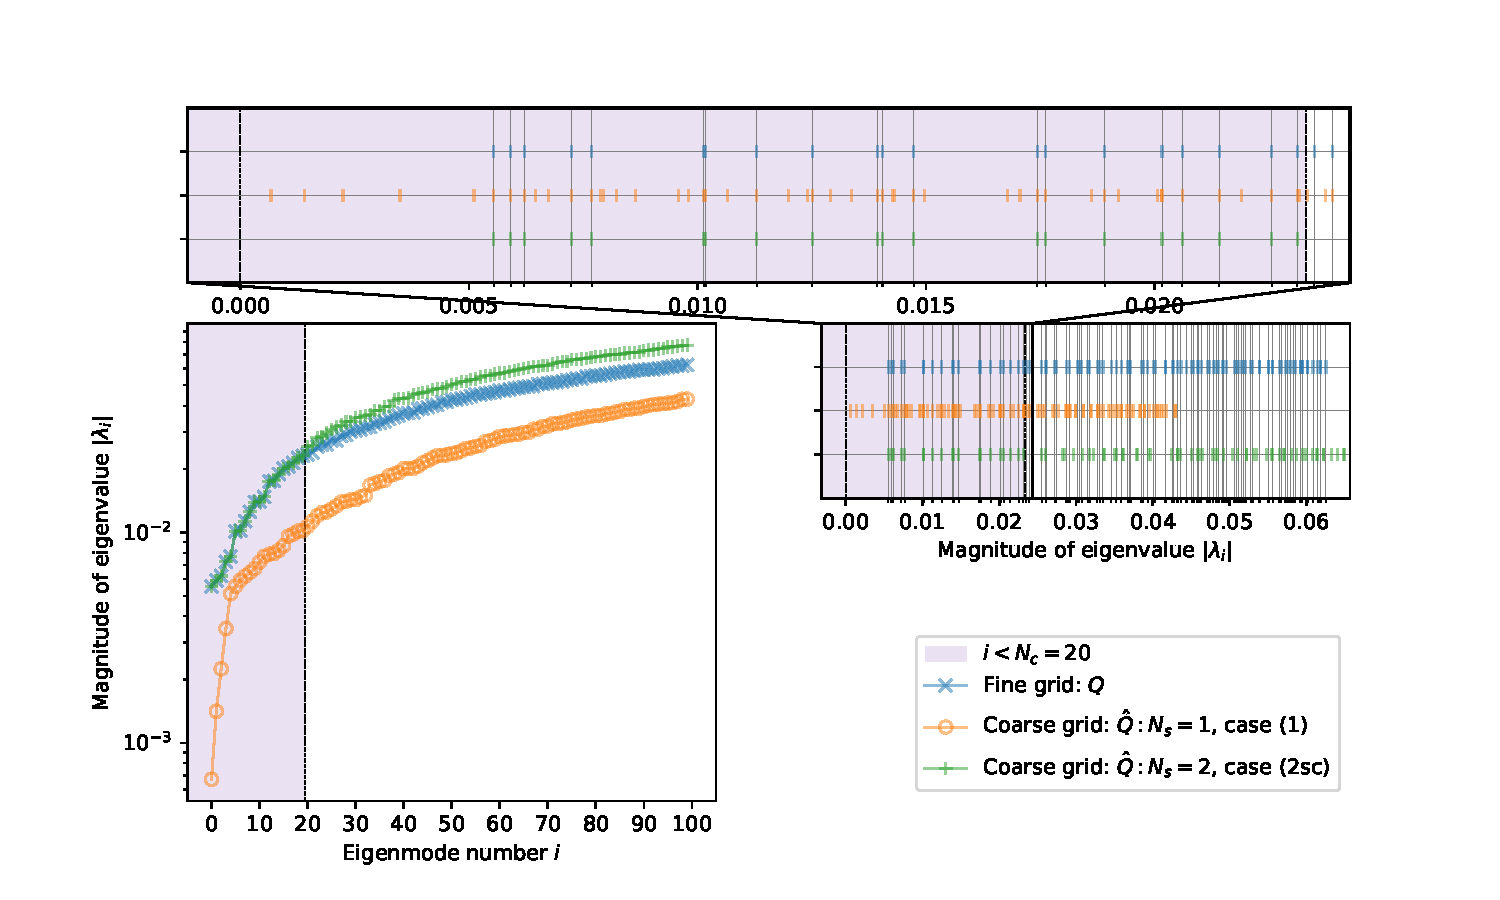
\includegraphics[width=1.0\linewidth]{\dir/img/eigenvalues_Nc20}
\caption{
Spectral study of coarse and fine Hermitian Dirac operators. Lower left: eigenvalue magnitude versus mode number, lower right: eigenvalue magnitude for comparison between the different operators, and top panel: zoom into the interesting region.
\takenfull
}
\label{fig:chirality:spectrum}
\end{figure}

\section{Numerical variance study}

The preserved chiral properties do not only have impact on the spectrum, but also the variance contribution of coarse subspaces.
\Cref{fig:chirality:variance} presents how it exhibits itself.
We can clearly see an immense benefit from the chiral property preservation as opposed to its absence.
Variance contributing to the large distance regime therefore originates from both chiral sectors.
The yellow data corresponds to the $i=1$ case in \ref{tab:spins}, whereas the yellow data to the $i=3$ case.
Even though subspace of the $i=3$ case is twice as large as the $i=1$ one, it is worth doing, not only for the condition of the coarse operator, but also for its variance contribution in the large distance.
\begin{figure}
\centering
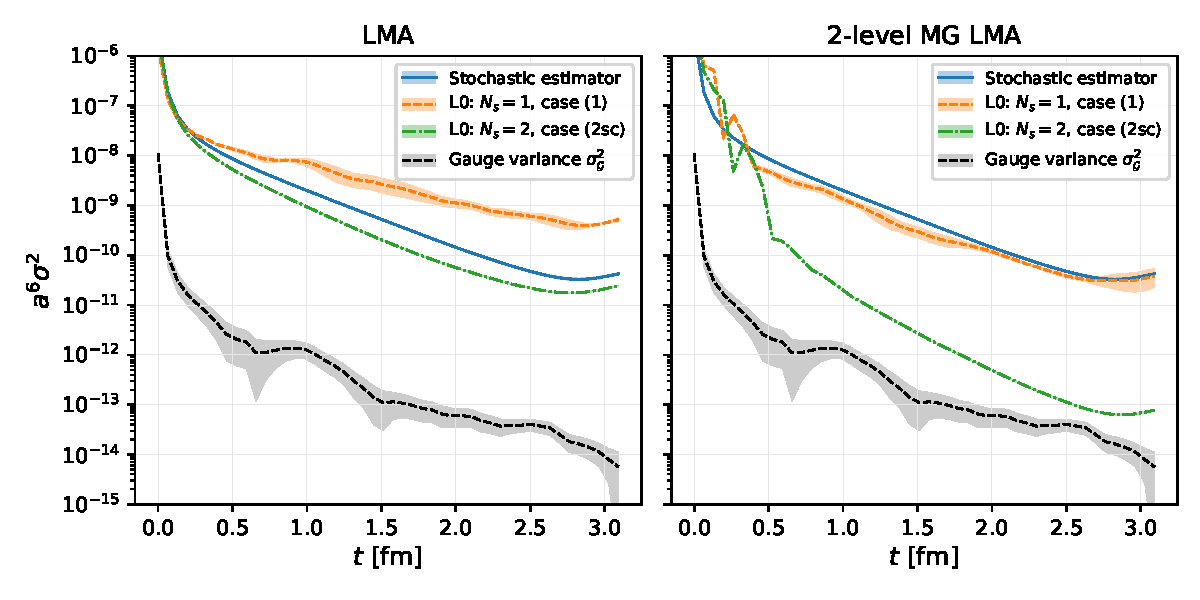
\includegraphics[width=1.0\linewidth]{\dir/img/chirality}
\caption{
Variance contribution of the \Ln{0}-term if all spin degrees of freedom are coarsened (yellow) as compared to when chiral properties are preserved (green).
Both LMA (left) and MG LMA (right) profit from these considerations.
\takenfull
}
\label{fig:chirality:variance}
\end{figure}

\section{Final conjecture}

We finish this chapter with a conjecture, motivated by the numerical and analytical studies above, from which we believe it is a sufficient condition for a well-behaved coarse-grid Dirac operator spectrum, suitable for coarse grid inversions as required by multigrid low-mode averaging.
\begin{conj}
Assume $K$ to be a positively stable, $\Gamma^{5}$-Hermitian operator acting on the fine-grid lattice, $K \colon \vslattice \rightarrow \vslattice$, not necessarily normal.
With Hermitian $P$ and $\Gamma^{5}$, we conjecture that if
\begin{equation} \label{eq:conj:chi}
\exists B \in \ggrp{GL}{N_s \Nc, \mathbb{C}} \; \colon \; \rho^5 = B \left( \chi^{5} \otimes \id_{\coarse{S}} \otimes \id_{\coarse{\idxcolor}} \right) B^{-1}
\end{equation}
for a change-of-basis matrix $B$, $\id_{\coarse{S}}$ is the identity of dimension either $1$ or $2$,
% and it holds
% \begin{equation} \label{eq:conj:modes}
% \forall i \; P \evec_i = \evec_i \;,
% \end{equation}
then chirality is preserved on the coarse lattice and
\begin{equation}
\kappa(\coarse{K}) \leq \kappa(K) \;.
\end{equation}
\end{conj}

Additionally we demand invariance of the $N_c$ lowest eigenmodes
\begin{equation} \label{eq:conj:modes}
\forall i \; P \evec_i = \evec_i \;,
\end{equation}
since this is a requirement coming from low-mode averaging.
%The invariance of the eigenmodes \cref{eq:conj:modes} is a requirement coming from low-mode averaging.
If not satisfied the subspace will not include the exact low modes resulting in a degraded variance reduction compared to low-mode averaging.
The particular form of the coarse chirality operator \cref{eq:conj:chi} on the other hand fulfills the statements in \cref{lemma:chirality:preservation:equiv,lemma:chirality:preservation:implications,lemma:svd:coarse,lemma:evals:coarse} while preserving the trace.

\section{Summary}
\label{sec:chirality:summary}

Chirality on the coarse subspaces is an important concept, and critical for MG LMA to be beneficial.
We have seen multiple ways to achieve this, all of which are equivalent in their outcome.
For Hermitian positive definite systems, we are guaranteed to have a better conditioned coarse operator, no matter how we coarsen.
We systemically relaxed assumptions to the operator, still upholding this guarantee.
On this way, preserving spectral properties of the fine operator to coarse grids is crucial.

\worktodo{todo}
